\documentclass{beamer}
\usepackage[utf8]{inputenc}
\usepackage[frenchb]{babel}
\usepackage[T1]{fontenc}
\usepackage{multicol}
\usepackage{lmodern}
\usepackage{vwcol}

\usetheme{Warsaw}

%\setbeamertemplate{headline}{}

\title[Rapport final de GRO]
      {Rapport final du projet de\\Graphes et Recherche opérationnelle}
\institute{Enseeiht}
\author
  [Ahlouche \and Arthaud \and Auguste
    \and Carton \and Forgione \and Wagner]
  {Maxence Ahlouche \and Maxime Arthaud \and Korantin Auguste
    \and Martin Carton \and Thomas Forgione \and Thomas Wagner}
\date{17 décembre 2013}

\begin{document}

\begin{frame}
  \titlepage
\end{frame}

\begin{frame}{Introduction}
  Blabla
\end{frame}

\section{Jeux}

\begin{frame}{Shifumi}
    \begin{block}{Équilibre de Nash}
        Équilibre de Nash~: jouer de manière aléatoire.
    \end{block}

    \begin{itemize}
        \item Chaines de Markov~: bat aisément un humain qui joue «~normalement~».
        \item Variantes~: reviennent au Shifumi classique si le nombre d'éléments est impair.
    \end{itemize}
\end{frame}

\section{Graphes}

\begin{frame}{Voyageur de commerce}
\end{frame}

\begin{frame}{Énoncé}
    Chercher un chemin passant par tous les sommets, de longueur minimale.
    \begin{itemize}
        \item cycle hamiltonien de coût minimal
        \item NP-complet
        \item méthodes approchées
    \end{itemize}
\end{frame}

\begin{frame}{Résolution approchée}
    \begin{block}{Heuristiques}
        Aller sur le nœud le plus près
    \end{block}

    \begin{block}{Recherche locale}
      \centering
      \begin{multicols}{2}
        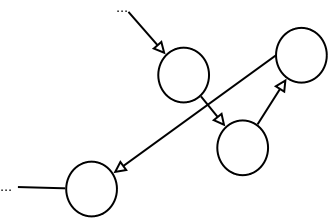
\includegraphics[width=0.3\textwidth]{../rapport/graphes/2opt1.png}

        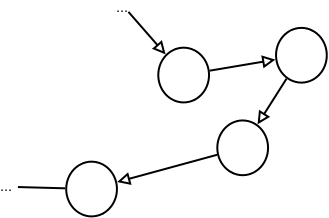
\includegraphics[width=0.3\textwidth]{../rapport/graphes/2opt2.png}
      \end{multicols}
    \end{block}
\end{frame}

\begin{frame}{Métaheuristiques}
    \begin{itemize}
        \item Recherche locale itérée
        \item Recherche tabou
        \item Recuit simulé
        \item Algorithmes génétiques
        \item Colonies de fourmis
    \end{itemize}
\end{frame}

\section{Programmation stochastique}
  \begin{frame}{Gare de péage}
    \begin{vwcol}[widths={0.6,0.4}, sep=.0cm, rule=0pt] 
      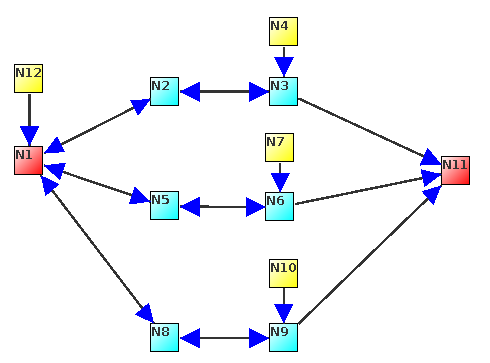
\includegraphics[width=6cm]{../../procstochs/img/3_files.png}

      \tiny
      \begin{itemize}
        \item $x[12] = random() < p_{cb}$
        \item $x[1] = random() < lambda$
        \item $x[2] =(x[2]>0)*(x[2]-1+d_{32})+d_{12}$
        \item $d_{12} = x[1]*d_{121}*(d_{21}<=d_{81})$
        \item $d_{23} = (x[2]>0)$
        \item $d_{32} = x[3]*(1-d_{43})$
        \item $x[3] = d_{23} + x[3]*(1-d_{23})*(1-d_{43})$
        \item $d_{311} = x[3]*d_{43}$
        \item $x[10] = random() < \frac 1 {p_{cb}/\mu_{cb}+(1-p_{cb})/\mu_{ncb}}$
      \end{itemize}
    \end{vwcol}
  \end{frame}
\end{document}
